%\documentclass[handout]{beamer} % Activate only if handout slides of presentation desired.
\documentclass[13.8pt]{beamer}

\usetheme{CambridgeUS}

% Packages
\usepackage[utf8]{inputenc}
\usepackage[T1]{fontenc}
\usepackage{amsmath}
\usepackage{graphicx}
\usepackage{eurosym}
\usepackage{hyperref}
\usepackage{amsmath}
\usepackage{graphicx}

\usepackage{tikz}
%\graphicspath{{../../2_Data/output}} % Sets the (relative) path of the figure directory

%%% 3) Tables
\usepackage{booktabs}  % Package optimizing the quality of LaTeX tables
\usepackage{longtable} % Necessary to represent LaTeX tables over multiple pages.
\usepackage{rotating}  % Necessary to represent full-page vertical regression tables 
\usepackage{multirow}  % Necessary to merge cells over multiple columns
\usepackage{makecell}  % Necessary to perform line breaks in a LaTeX table
\usepackage{tabularx}  % Needed to e.g. write long text in cells and get automatic linebreak.
\usepackage{caption}
\usepackage{adjustbox} % needed to adjust the tables to textwidth.
\usepackage{tcolorbox}
\graphicspath{ {./graphs/} }
\setbeamercolor{bgcolor}{fg=white,bg=orange} 


\setlength{\unitlength}{1.2cm}
\setcounter{tocdepth}{2} 
\setbeamertemplate{footline}
{
	\leavevmode%
	\hbox{%
		\begin{beamercolorbox}[wd=0.4\paperwidth,ht=2.25ex,dp=1ex,center]{title in head/foot}%
			\usebeamerfont{author in head/foot}\today
		\end{beamercolorbox}
		
		\begin{beamercolorbox}[wd=.3\paperwidth,ht=2.25ex,dp=1ex,center]{author in head/foot}%
			\usebeamerfont{title in head/foot} Bailing out Firms Through Banks
		\end{beamercolorbox}
		%
		\begin{beamercolorbox}[wd=.3\paperwidth,ht=2.25ex,dp=1ex,center]{title in head/foot}%
			\usebeamerfont{title in head/foot}
			\insertframenumber{} / \inserttotalframenumber\hspace*{1ex}
		\end{beamercolorbox}}%


	\vskip0pt%
}

\setbeamertemplate{headline}
{
	\leavevmode%
	\hbox{%
		\begin{beamercolorbox}[wd=0.5\paperwidth,ht=2.25ex,dp=1ex,center]{title in head/foot}%
			\usebeamerfont{author in head/foot} \insertsectionhead
		\end{beamercolorbox}
		
		\begin{beamercolorbox}[wd=0.5\paperwidth,ht=2.25ex,dp=1ex,center]{author in head/foot}%
			\usebeamerfont{title in head/foot} \insertsubsectionhead
		\end{beamercolorbox}}
		%


	\vskip0pt%
}

\usepackage{enumitem}
\usepackage{xcolor}
\usepackage{tikz}
\usetikzlibrary{shadows}
\setbeamertemplate{navigation symbols}{}
%\beamertemplatesolidbackgroundcolor{black!5}
%\setbeamercovered{transparent}


\newcommand*{\MyBall}{\tikz \draw [baseline, ball color=red, draw=red] circle (2.5pt);}

%-------------------------------------------------------------




%-------------------------------------------------------------

\begin{document}
	
\title{Bailing out Firms Through Banks Jan is the best}
\author{Chunjie Wang and Martin Waibel (2020)}
\date{\today}

 \renewcommand*\inserttotalframenumber{14	}

\begin{frame}
\maketitle
\end{frame}


\section{Introduction}
\subsection{Motivation}
\begin{frame}
\frametitle{Motivation}

\begin{itemize}[label={\MyBall}]
	\pause
	\item Corporate liquidity management is of crucial importance for firms during the COVID-19 pandemic.

	\pause
	\item Most governments around the world introduced forms of credit relief programs to bridge funding gaps in the corporate sector.

	\pause
	\item Large existing body of literature focuses on optimal government bailout of \textit{financial} institutions.
	
	\pause
	\item Less is known about how non-financial firms should be bailed out.
\end{itemize}

$\implies$ Theory linking federal bailouts with the banking and firm sector.

\end{frame}

\begin{frame}
\frametitle{Relevant Questions}

\begin{itemize}[label={\MyBall}]
	\pause
	\item How can a government bail out firms via the banking sector?
	\pause
	\item At what costs does the bailout come for the government?
	\pause
	\item What changes in case the liquidity shock is private information to the bank and the firm?
	\pause
	\item How should the government decide on whether or not to bail out a firm?
\end{itemize}
\end{frame}

\begin{frame}
\frametitle{Contribution and Results}
\end{frame}

\begin{frame}
\frametitle{Literature}
\textbf{\large\underline{Government bailouts:}}\\ 
Acharya et al. (2014), Blau et al. (2013), Faccio et al. (2006), Gorton and Huang (2004), Diamond and Rajan (2002), Lewrick et al. (2014), Ennis and Keister (2009) \\
\vspace{0.5cm}
\textbf{\large\underline{Corporate liquidity management:}}\\
Holström and Tirole (1997), Tirole (2006), Yun (2009), Campello et al. (2011), Jimenez et al. (2009), Demiroglu and James (2011)


\vspace{1cm}
\textbf{\large\underline{Credit access during Covid-19:}}\\
Banerjee et al. (2020), Bartik et al. (2020), Balduzzi et al. (2020), Dursun-de Neef et al. (2020)


\end{frame}


\section{Model}
\subsection{Model setup}
\begin{frame}
\frametitle{XXX}
\end{frame}

\begin{frame}
\frametitle{XXX}
\end{frame}

\section{Analysis}
\subsection{XXX}
\begin{frame}
\frametitle{XY}
\end{frame}

\begin{frame}
\frametitle{XY}
\end{frame}



\section{Model}
\subsection{Model setup}
\begin{frame}
\frametitle{Basic Setup: Contracted Liquidity Shock (Tirole, 2006)}
\begin{itemize}[label={\MyBall}]
	\item $t\in \{ 0,1,2\}$
	\item Two agents: firm (endowment $A$) and investor
	\item One project: 
		\begin{itemize}
		\item $t=0$: upfront investment $I$;
		\item $t=1$: liquidity shock $\rho$ randomly drawn from cdf $F(\rho)$;
		\item $t=2$: the project yields
							$0$ if $\rho$ is not committed;
							$p_H R$ if $\rho$ is committed and firm exerts effort;
							$p_L R$ if $\rho$ is committed and firm shirks.							
	\end{itemize}
	\item Moral hazard: effort is not contractible and shirking yields private benefit $B$ to the firm.  
	
\end{itemize}

\end{frame}

\begin{frame}
\frametitle{Basic Setup: Contracted Liquidity Shock (Tirole, 2006)}
\begin{itemize}[label={\MyBall}]
\item The financing contract at $t=0$ needs to be incentive compatible: the firm requires $p_H\frac{B}{\Delta p}$ to exert effort.
\item The contract at $t=0$ also states the maximum liquidity shock $\rho ^*$ at $t=1$ that the investor agrees to finance.
\item Pledgeable in come to bank in a competitive credit market is thus \begin{align*}
    \mathcal{P}(\rho ^*)=F(\rho ^*)p_H\left( R-\frac{B}{\Delta p}\right)-\int ^{\rho ^*}_0 \rho f(\rho)d\rho=I-A
\end{align*}
\item The expected payoff to the firm is \begin{equation*}
    NPV_{firm}(\rho ^*)=U_{firm}(\rho ^*)=F(\rho ^*)p_HR-\left( I+\int ^{\rho ^*}_0 \rho f(\rho)d\rho \right)
\end{equation*}

\end{itemize}

\end{frame}

\begin{frame}
\frametitle{Basic Setup: Contracted Liquidity Shock (Tirole, 2006)}
\begin{itemize}[label={\MyBall}]
\item $U_{firm}(\rho ^*)$ peaks at $\rho *=p_HR$ and $\mathcal{P}(\rho ^*)$ peaks at $\rho *=p_H(R-\frac{B}{\Delta p})$.
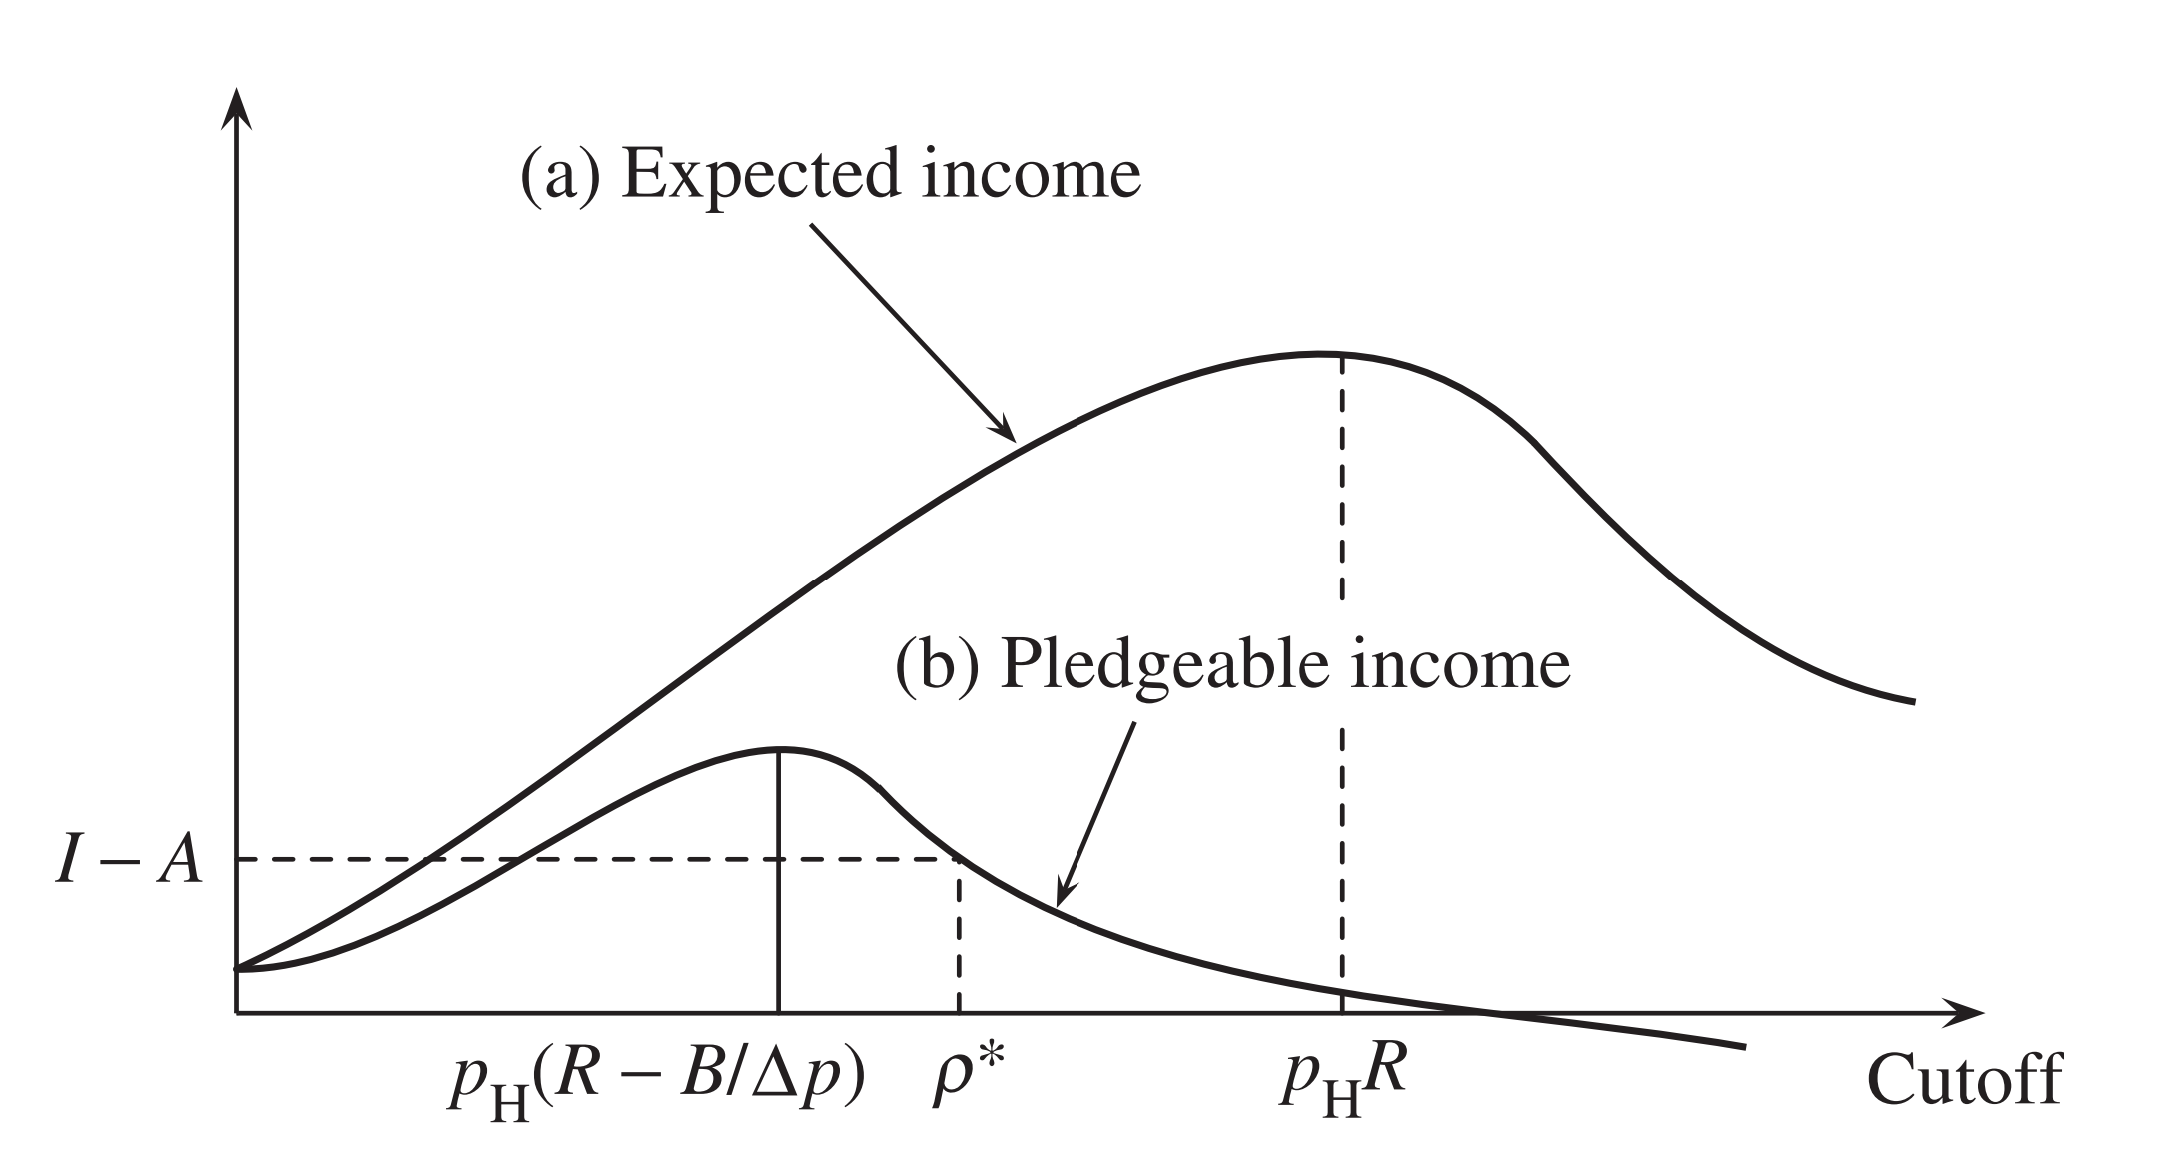
\includegraphics[scale=0.4]{Tirole}

\item if $\mathcal{P}(p_HR)\geq I-A$: $\rho^*$ is set to equal $p_HR$;
\item if $\mathcal{P}(p_HR)< I-A\leq  \mathcal{P}\left(p_H\left(R-\frac{B}{\Delta p} \right) \right)$: $\rho ^* \in \left[p_H(R-\frac{B}{\Delta p}), p_HR \right[$ solves $\mathcal{P}(\rho ^*)=I-A$


\end{itemize}

\end{frame}


\begin{frame}
\frametitle{Basic Setup: Contracted Liquidity Shock (Tirole, 2006)}
\begin{itemize}[label={\MyBall}]
\item $ \rho ^* \in [p_H(R-\frac{B}{\Delta p}),  p_HR]$ implies the firm needs to plan its liquidity management at $t=0$ according to either of the following specifications or any combination of them:
\vspace{0.5cm}
\begin{itemize}[label={\MyBall}]
\item \textbf{secure a line of credit of $\rho^*$ with no right to dilute the existing share by issuing new claims at $t=1$;}
    \item secure a credit line of $\rho^*-p_H(R-\frac{B}{\Delta p})$ with a right to dilute the existing share at $t=1$;
\end{itemize}
\vspace{0.5cm}
\item It turns out which specification the firm decides to follow does not matter in our model, thus throughout the paper, we assume the first case. 


\end{itemize}
\end{frame}

\begin{frame}
\frametitle{Government Intervention and New Moral Hazard}
\begin{itemize}[label={\MyBall}]
\item An aggregate liquidity shock $\rho>\rho^*$ hits all firms: government with deep pocket intervenes at $t=1$.
\item The government can only monitor the firm through the investor.
\vspace{0.5cm}
\item The firm at $t=1$, if not monitored, chooses between:
\begin{itemize}[label={\MyBall}]
\item \textbf{reinvest:} invest government liquidity together with the credit line contracted with the investor;
\item \textbf{default:} consume the government injection.
\end{itemize}


\end{itemize}
\end{frame}

\begin{frame}
\frametitle{Government Intervention and New Moral Hazard}

\begin{table}[H]
\centering
\caption{Cashflows Upon Federal Liquidity Injection}
\resizebox{3in}{!}{\begin{tabular}{lcccc}
\hline
Decision &  Agent            & $t=0$      & $t=1$     & $t=2$  \\ \hline
\multirow{2}{*}{reinvest} & Firm & $-A$     &   0    & $p_H\frac{B}{\Delta p}$ \\
& Bank     & $-(I-A)$ & $-\rho$ * & $p_H\left( R-\frac{B}{\Delta p}\right)$ \\ \hline
\hline
%t            & $0$      & $1$     & $2$  \\ \hline
\multirow{2}{*}{default}& Firm & $-A$     & $+(\rho-\rho ^*)$       & 0 \\
& Bank     & $-(I-A)$ & 0  & 0 \\ \hline
\end{tabular}}
\end{table}
\begin{itemize}[label={\MyBall}]

\item $ \rho ^* \in [p_H(R-\frac{B}{\Delta p}),  p_HR] \implies$ \textbf{investor does not have incentive to monitor regardless of $\rho$}, he would rather the project go south.
\vspace{0.5cm}
\item When $\rho ^*+\frac{p_HB}{\Delta p}\geq \rho>\rho ^*$, the firm reinvests;
\item When $\rho>\rho^*+\frac{p_HB}{\Delta p}$, the firm defaults, a moral hazard between firm and government emerges.

\end{itemize}
\end{frame}


\begin{frame}
\frametitle{Fiscal Cost of Intervention}
\begin{itemize}[label={\MyBall}]
\item There is no moral hazard between the government and the firm when $\rho$ is small.
\item Moral hazard emerges when liquidity shock $\rho$ surpasses a point ($\rho^*+\frac{p_HB}{\Delta p}$).
\item To overcome the problem, the government has to incentivize the investor by paying him $D$ to monitor the firm:
\begin{align*}
D=\rho ^*-p_H(R-\frac{B}{\Delta p})    
\end{align*}
\vspace{0.5cm}
\item in case of effective government intervention, such moral hazard \textbf{causes a discontinuous increase} $D$ in the government spending and investor utility at a cutoff.

\end{itemize}
\end{frame}


\begin{frame}
\frametitle{Fiscal Cost of Intervention}
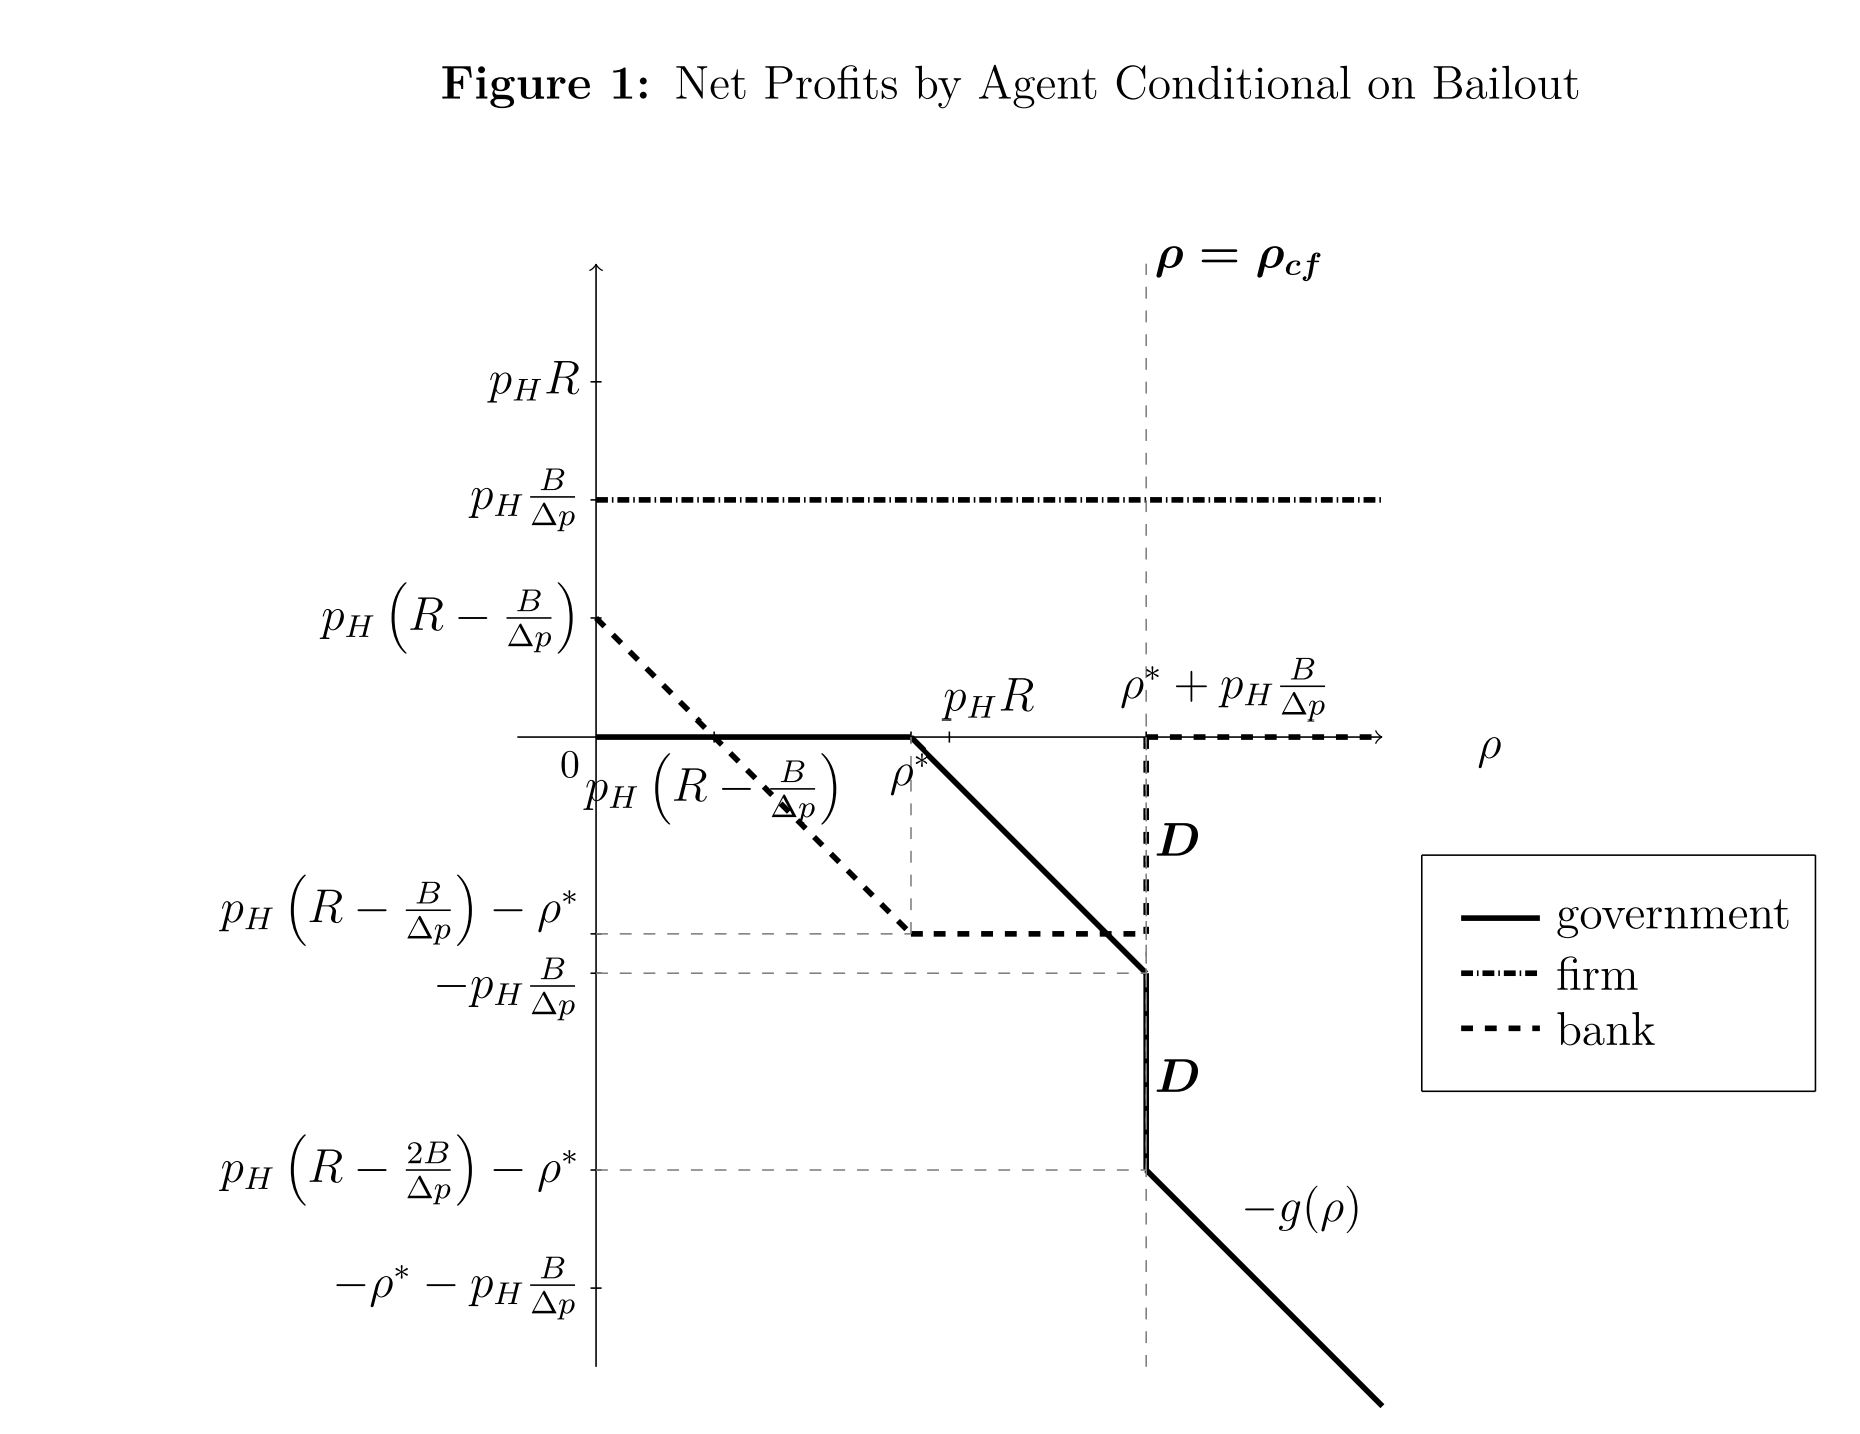
\includegraphics[scale=0.6]{utility1}
\end{frame}

\begin{frame}
\frametitle{Externality}
\begin{itemize}[label={\MyBall}]
\item Bailing out firms is always financially costly to the government, so why would a government intervene?
\item Each firm provides a positive externality $\frac{\phi}{N} > 0$, where $N$ is the total number of firms in the economy. In case of aggregate shock that threats the whole economy, the government evaluates $\phi$ against $g(\rho)$ 
\vspace{1cm}
\item \textbf{Policy Recommendation 1:} \textit{The government decides to inject liquidity in response to a liquidity shock of size $\rho$ whenever $\phi-g(\rho)>0 \iff \rho<g^{-1}(\phi)$ assuming that the government is able to observe the liquidity shock.}
\end{itemize}
\end{frame}

\begin{frame}
\frametitle{Over-Report Tendency}
\begin{itemize}[label={\MyBall}]
\item So far, we have assumed that the government is able to observe the realized liquidity shock $\rho$ at $t=1$.
\item Yet it is particularly likely that the true liquidity shock $\rho_t$ is private information to the firm and the investor.
\item This informational asymmetry allows the firm-investor pair to over-report the actual liquidity shock as $\rho_{r} = \rho_{t}+\sigma$ for some $\sigma \geq 0$ so as to jointly realize extra payoff.
\item The problem is aggravated around the cutoff $\rho_{cf}$. This is because  over-reporting for some $\rho_t$ slightly below $\rho_{cf}$ could lead to a discontinuous increase in fiscal costs.

\end{itemize}
\end{frame}

\begin{frame}
\frametitle{Over-Report Tendency}
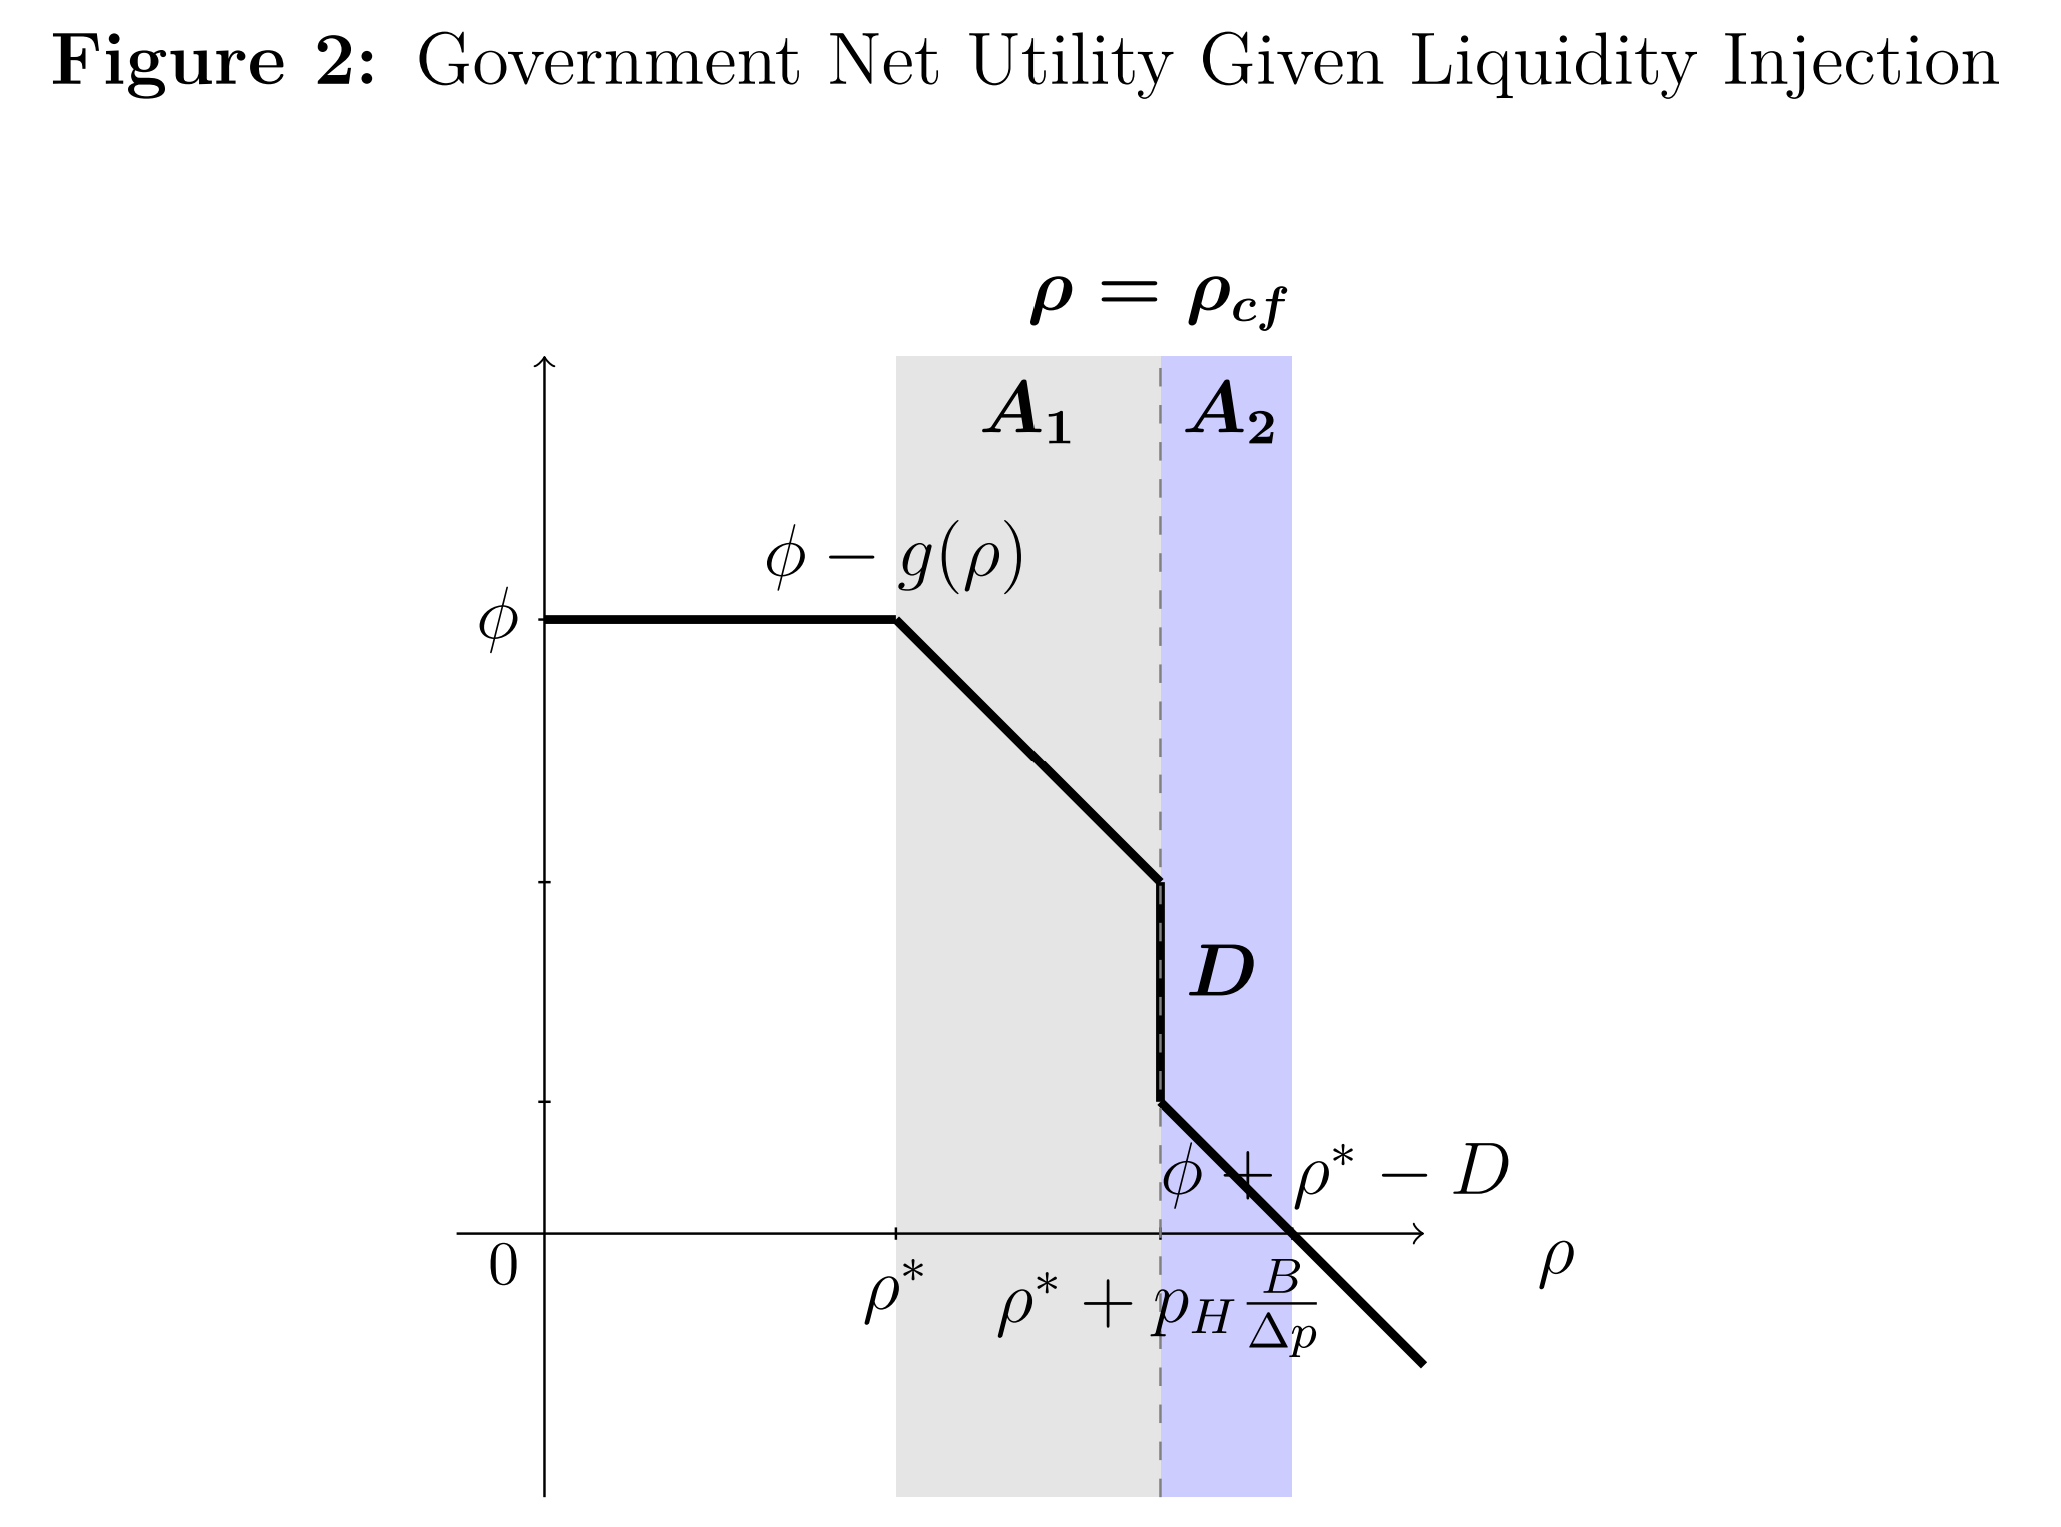
\includegraphics[scale=0.4]{utility2}
\begin{itemize}[label={\MyBall}]

\item The moral hazard between the government and the firm only exists in $A_2$ but not in $A_1$;
\item A bank-firm pair with $\rho_t \in A_1$ has incentives to report a higher shock and pretend to be in $A_2$ in order to exploit $D$
\end{itemize}
\end{frame}

\begin{frame}
\frametitle{Over-Report Tendency}
\begin{itemize}[label={\MyBall}]

\item Knowing the over-report tendency, how can the government improves the situation? 
\item Denote $\tilde{\rho}$ as the optimal policy cutoff based on which the government decides about the size of the liquidity injection.
\begin{gather*}
    g(\rho_r) = \begin{cases} 
      \rho_r-\rho^* & \text{for}\,\, \rho^* < \rho \leq \tilde{\rho} \\
      \rho_r-\rho^*+D & \text{for}\,\,\rho > \tilde{\rho}
   \end{cases}
\end{gather*}
\item Our goal: to find $\tilde{\rho}$ that causes the least loss to the government compared to a perfect world without over-report tendency.
\end{itemize}
\end{frame}

\begin{frame}
\frametitle{Over-Report Tendency}
\begin{itemize}[label={\MyBall}]

\item Observing $\rho_r$, the government forms an estimate of $\sigma=\rho_r-\rho_t$, denoted as $\psi$, which is continuously distributed with cdf $H(\psi)$.
\item If the government grants $\rho_r-\rho^*+D$, the expected loss (compared to perfect world) is $\int h(\psi)\psi \,\,d\psi+\mathbb{P}(\rho_r-\psi \leq \rho_{cf})D$, denoted as \textcolor{red}{\textit{type I loss}}. 
\item If the government only grants $\rho_r-\rho^*$, the expected loss is $\int h(\psi)\psi \,\,d\psi+\mathbb{P}(\rho_r-\psi > \rho_{cf})(\phi-D)$, denoted as \textcolor{red}{\textit{type II loss}}. 
\item By definition of $\tilde{\rho}$, it solves when the two types loss equalize.
\end{itemize}
\end{frame}

\begin{frame}
\frametitle{Over-Report Tendency}
\begin{itemize}[label={\MyBall}]

\item Solving the problem:
\begin{align*}
         \tilde{\rho}&=\rho_{cf}+H^{-1}\left( \frac{D}{\phi} \right).
\end{align*}
\item \textbf{Policy Recommendation 2:} \textit{In case of informational asymmetries between the bank-firm pair and the government with respect to the actual liquidity shock $\rho_t$ the fiscal authority should set $\tilde{\rho}=\rho_{cf}+H^{-1}\left( \frac{D}{\phi} \right)$.}
\end{itemize}
\end{frame}

\section{Analysis}
\subsection{Fiscal Cost of Intervention}




\begin{frame}
\frametitle{Extension}

\begin{itemize}[label={\MyBall}]

	\item Idea: In the US banks are forced to keep a minimum of 5\% of the credit risk on their balance sheet. 

	\item Show adjusted table on page 10 

	\item In the current version of the model, whether or not the banks are exposed to part of the credit risk doesn't change their monitoring incentives because the IC and PC need to be fulfilled and the payoff structure cannot be altered. 

	\item Question: How can we move to a more accurate description of reality by allowing for repayment of

\end{itemize}
\end{frame}

\section{Conclusion}
\begin{frame}
\frametitle{Conclusion}
Model of government bailout of firms through financial intermediaries
	\begin{itemize}[label={\MyBall}]
		\item Aggregate liquidity shock exceeds firms' credit lines.\\
		$\implies$ Requires externality-valuing government to make a decision about liquidity injections.
		\pause
		\item Federal liquidity injection via financial intermediaries creates a discontinuous increase in fiscal costs due to moral hazard.
		\pause
		\item Private information about the size of the liquidity shock  aggravates the moral hazard problem locally.
		\pause
		\item Government intervention is costly but not substitutable by the financial intermediaries.
	\end{itemize}

\end{frame}

\section{Appendix}
\begin{frame}
\frametitle{XXX}
\end{frame}




\end{document}